%% This is the ctufit-thesis example file. It is used to produce theses
%% for submission to Czech Technical University, Faculty of Information Technology.
%%
%% Get the newest version from
%% https://gitlab.fit.cvut.cz/theses-templates/FITthesis-LaTeX
%%
%%
%% Copyright 2021, Eliska Sestakova and Ondrej Guth
%%
%% This work may be distributed and/or modified under the
%% conditions of the LaTeX Project Public Licenese, either version 1.3
%% of this license or (at your option) any later version.
%% The latest version of this license is in
%%  https://www.latex-project.org/lppl.txt
%% and version 1.3 or later is part of all distributions of LaTeX
%% version 2005/12/01 or later.
%%
%% This work has the LPPL maintenance status `maintained'.
%%
%% The current maintainer of this work is Ondrej Guth.
%% Contact ondrej.guth@fit.cvut.cz for bug reports.
%% Alternatively, submit bug reports into the tracker at
%% https://gitlab.fit.cvut.cz/theses-templates/FITthesis-LaTeX/issues
%%
%%

%%%%%%%%%%%%%%%%%%%%%%%%%%%%%%%%%%%%%%%%%
% CLASS OPTIONS
% language: czech/english/slovak
% thesis type: bachelor/master/dissertation
% colour: bw for black&white OR no option for default colour scheme
%%%%%%%%%%%%%%%%%%%%%%%%%%%%%%%%%%%%%%%%%
\documentclass[english,master,unicode]{ctufit-thesis}

%%%%%%%%%%%%%%%%%%%%%%%%%%%%%%%%%%
% FILL IN THIS INFORMATION
%%%%%%%%%%%%%%%%%%%%%%%%%%%%%%%%%%
\ctufittitle{A system for signals manipulation on the automotive ethernet} % replace with the title of your thesis
\ctufitauthorfull{Ing. Oleksandr Korotetskyi} % replace with your full name (first name(s) and then family name(s) / surname(s)) including academic degrees
\ctufitauthorsurnames{Korotetskyi} % replace with your surname(s) / family name(s)
\ctufitauthorgivennames{Oleksandr} % replace with your first name(s) / given name(s)
\ctufitsupervisor{Ing. Martin Štěpánek} % replace with name of your supervisor/advisor (include academic degrees)
\ctufitdepartment{Department of Software Engineering} % replace with the department of your defence
\ctufityear{2023} % replace with the year of your defence
\ctufitdeclarationplace{Prague, Czech Republic} % replace with the place where you sign the declaration
\ctufitdeclarationdate{\today} % replace with the date of signature of the declaration
\ctufitabstractCZE{Fill in abstract of this thesis in Czech language. Class aptent taciti sociosqu ad litora torquent per conubia nostra, per inceptos hymenaeos. Cras pede libero, dapibus nec, pretium sit amet, tempor quis. Sed vel lectus. Donec odio tempus molestie, porttitor ut, iaculis quis, sem. Suspendisse sagittis ultrices augue.}
\ctufitabstractENG{Fill in abstract of this thesis in English language. Class aptent taciti sociosqu ad litora torquent per conubia nostra, per inceptos hymenaeos. Cras pede libero, dapibus nec, pretium sit amet, tempor quis. Sed vel lectus. Donec odio tempus molestie, porttitor ut, iaculis quis, sem. Suspendisse sagittis ultrices augue.}
\ctufitkeywordsCZE{enter, commma, separated, list, of, keywords, in, CZECH}
\ctufitkeywordsENG{enter, commma, separated, list, of, keywords, in, ENGLISH}
%%%%%%%%%%%%%%%%%%%%%%%%%%%%%%%%%%
% END FILL IN
%%%%%%%%%%%%%%%%%%%%%%%%%%%%%%%%%%

%%%%%%%%%%%%%%%%%%%%%%%%%%%%%%%%%%
% CUSTOMIZATION of this template
% Skip this part or alter it if you know what you are doing.
%%%%%%%%%%%%%%%%%%%%%%%%%%%%%%%%%%

\RequirePackage{iftex}[2020/03/06]
\iftutex % XeLaTeX and LuaLaTeX
    \RequirePackage{ellipsis}[2020/05/22] %ellipsis workaround for XeLaTeX
\else
    \RequirePackage[utf8]{inputenc}[2018/08/11] %this file encoding
    \RequirePackage{lmodern}[2009/10/30] % vector flavor of Computer Modern font
\fi

% hyperlinks
\RequirePackage[pdfpagelayout=TwoPageRight,colorlinks=false,allcolors=decoration,pdfborder={0 0 0.1}]{hyperref}[2020-05-15]

% uncomment the following to hide all hyperlinks
% \RequirePackage[pdfpagelayout=TwoPageRight,hidelinks]{hyperref}[2020-05-15]

\RequirePackage{pdfpages}[2020/01/28]

\setcounter{secnumdepth}{4} % numbering sections; 4: subsubsection



%%%%%%%%%%%%%%%%%%%%%%%%%%%%%%%%%%
% CUSTOMIZATION of this template END
%%%%%%%%%%%%%%%%%%%%%%%%%%%%%%%%%%
\newcommand\boldred[1]{\textcolor{red}{\textbf{#1}}}        % attetion
\newcommand\boldblue[1]{\textcolor{blue}{\textbf{#1}}}      % comment
\newcommand\boldgreen[1]{\textcolor{green}{\textbf{#1}}}    % todo
\newcommand\boldorange[1]{\textcolor{orange}{\textbf{#1}}}  % literature required


%%%%%%%%%%%%%%%%%%%%%%
% DEMO CONTENTS SETTINGS
% You may choose to modify this part.
%%%%%%%%%%%%%%%%%%%%%%
\usepackage{tabularx}
\usepackage{adjustbox}
\usepackage{graphicx}
\usepackage{multirow}
\usepackage{longtable}
\usepackage{dirtree}
\usepackage{enumitem}
\usepackage{lipsum,tikz}
\usepackage{csquotes}
\usepackage[style=iso-numeric]{biblatex}
\addbibresource{text/bib-database.bib}
\usepackage{listings} % typesetting of sources
% \usepackage{minted} % typesetting of sources

%theorems, definitions, etc.
\theoremstyle{plain}
\newtheorem{theorem}{Věta}
\newtheorem{lemma}[theorem]{Tvrzení}
\newtheorem{corollary}[theorem]{Důsledek}
\newtheorem{proposition}[theorem]{Návrh}
\newtheorem{definition}[theorem]{Definice}
\theoremstyle{definition}
\newtheorem{example}[theorem]{Příklad}
\theoremstyle{remark}
\newtheorem{note}[theorem]{Note}
\newtheorem*{note*}{Poznámka}
\newtheorem{remark}[theorem]{Remark}
\newtheorem*{remark*}{Pozorování}
\numberwithin{theorem}{chapter}
%theorems, definitions, etc. END
%%%%%%%%%%%%%%%%%%%%%%
% DEMO CONTENTS SETTINGS END
%%%%%%%%%%%%%%%%%%%%%%

\begin{document} 
\frontmatter\frontmatterinit % do not remove these two commands

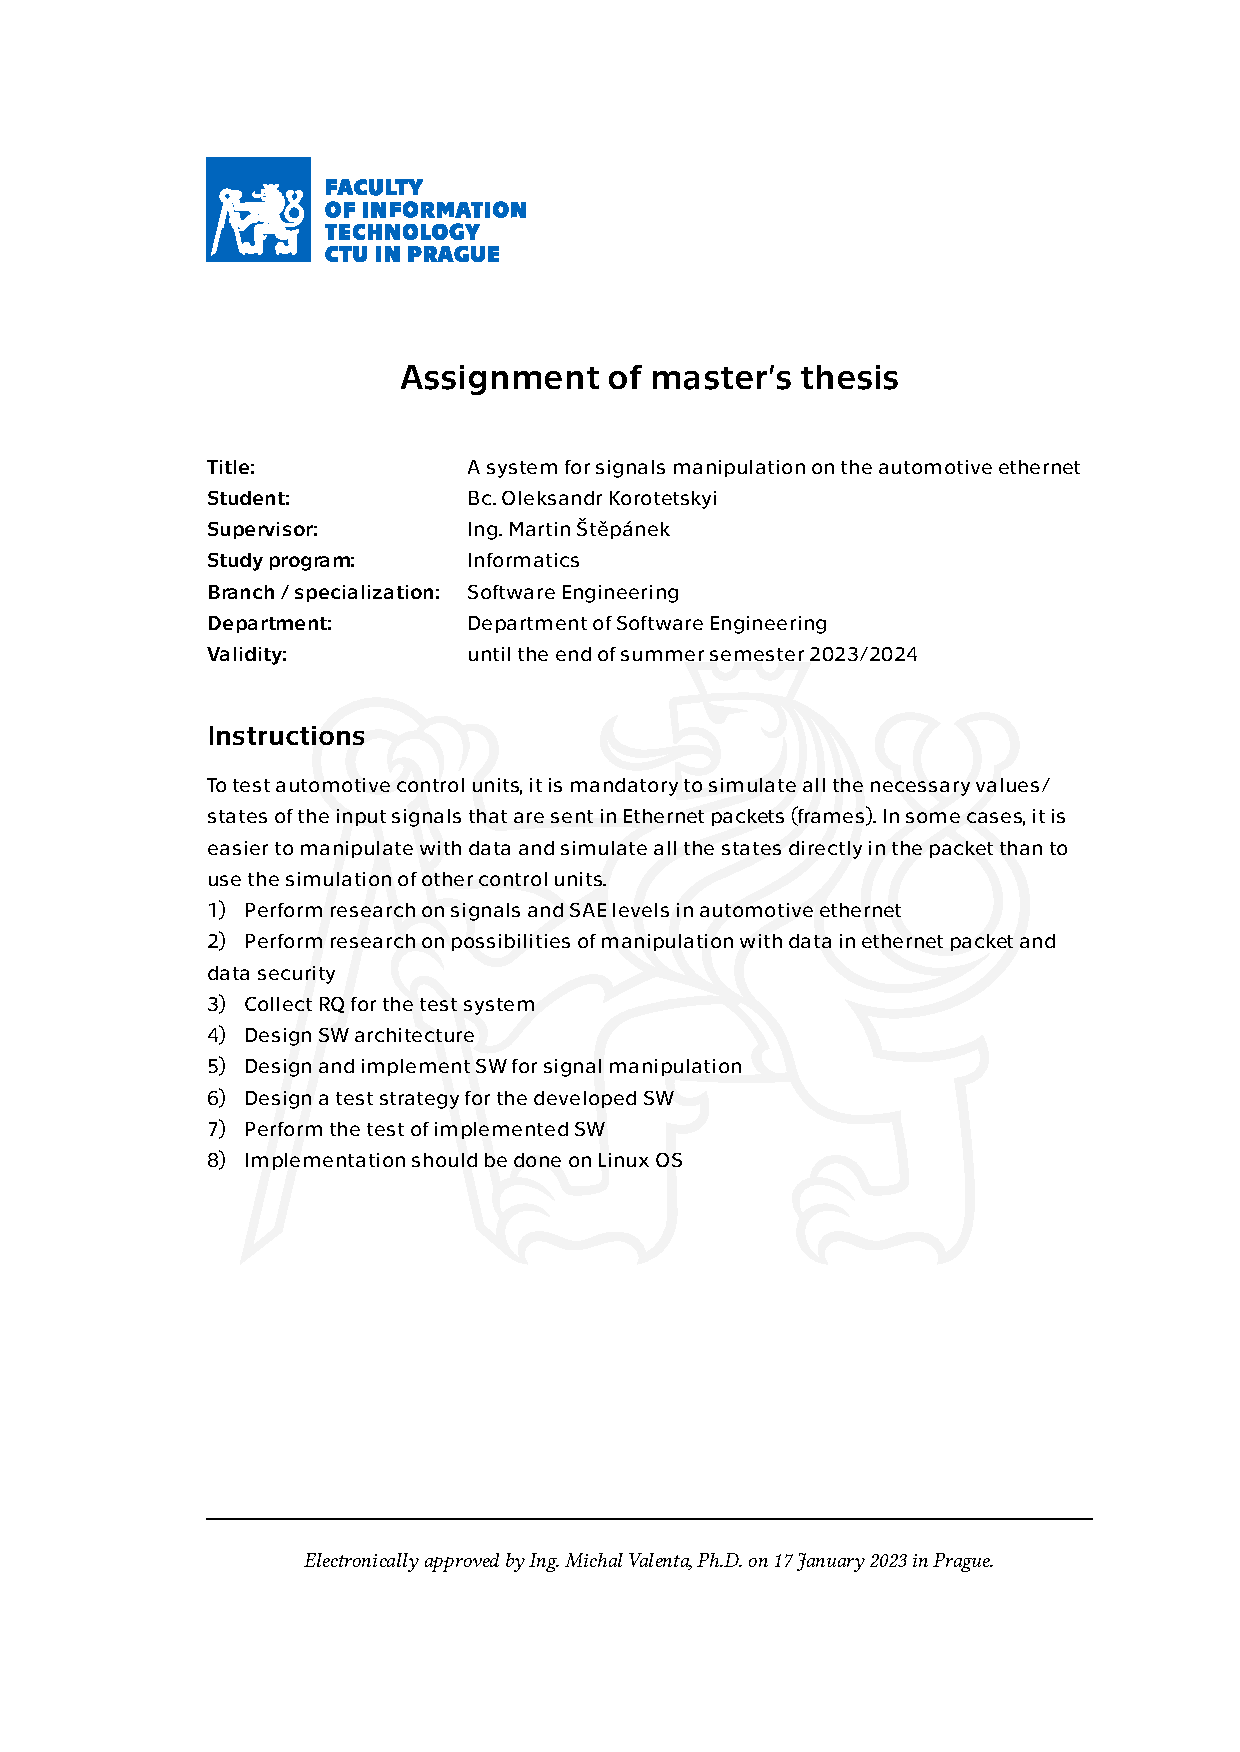
\includepdf[pages={1-}]{korotole-assignment.pdf} % replace that file with your thesis assignment provided by study office

\thispagestyle{empty}\cleardoublepage\maketitle % do not remove these three commands

\imprintpage % do not remove this command

\tableofcontents % do not remove this command
%%%%%%%%%%%%%%%%%%%%%%
% list of other contents: figures, tables, code listings, algorithms, etc.
% add/remove commands accordingly
%%%%%%%%%%%%%%%%%%%%%%
\listoffigures % list of figures
\begingroup
\let\clearpage\relax
\listoftables % list of tables
\lstlistoflistings % list of source code listings generated by the listings package
% \listoflistings % list of source code listings generated by the minted package
\endgroup
%%%%%%%%%%%%%%%%%%%%%%
% list of other contents END
%%%%%%%%%%%%%%%%%%%%%%

%%%%%%%%%%%%%%%%%%%
% ACKNOWLEDGMENT
% FILL IN / MODIFY
% This is a place to thank people for helping you. It is common to thank your supervisor.
%%%%%%%%%%%%%%%%%%%
\begin{acknowledgmentpage}
	Chtěl bych poděkovat především sit amet, consectetuer adipiscing elit. Curabitur sagittis hendrerit ante. Class aptent taciti sociosqu ad litora torquent per conubia nostra, per inceptos hymenaeos. Cras pede libero, dapibus nec, pretium sit amet, tempor quis. Sed vel lectus. Donec odio tempus molestie, porttitor ut, iaculis quis, sem. Suspendisse sagittis ultrices augue.
\end{acknowledgmentpage} 
%%%%%%%%%%%%%%%%%%%
% ACKNOWLEDGMENT END
%%%%%%%%%%%%%%%%%%%


%%%%%%%%%%%%%%%%%%%
% DECLARATION
% FILL IN / MODIFY
%%%%%%%%%%%%%%%%%%%
% INSTRUCTIONS
% ENG: choose one of approved texts of the declaration. DO NOT CREATE YOUR OWN. Find the approved texts at https://courses.fit.cvut.cz/SFE/download/index.html#_documents (document Declaration for FT in English)
% CZE/SLO: Vyberte jedno z fakultou schvalenych prohlaseni. NEVKLADEJTE VLASTNI TEXT. Schvalena prohlaseni najdete zde: https://courses.fit.cvut.cz/SZZ/dokumenty/index.html#_dokumenty (prohlášení do ZP)
\begin{declarationpage}
FILL IN ACCORDING TO THE INSTRUCTIONS. VYPLŇTE V SOULADU S POKYNY. Lorem ipsum dolor sit amet, consectetuer adipiscing elit. Curabitur sagittis hendrerit ante. Class aptent taciti sociosqu ad litora torquent per conubia nostra, per inceptos hymenaeos. Cras pede libero, dapibus nec, pretium sit amet, tempor quis. Sed vel lectus. Donec odio tempus molestie, porttitor ut, iaculis quis, sem. Suspendisse sagittis ultrices augue. Donec ipsum massa, ullamcorper in, auctor et, scelerisque sed, est. In sem justo, commodo ut, suscipit at, pharetra vitae, orci. Pellentesque pretium lectus id turpis.

Lorem ipsum dolor sit amet, consectetuer adipiscing elit. Curabitur sagittis hendrerit ante. Class aptent taciti sociosqu ad litora torquent per conubia nostra, per inceptos hymenaeos. Cras pede libero, dapibus nec, pretium sit amet, tempor quis. Sed vel lectus. Donec odio tempus molestie, porttitor ut, iaculis quis, sem. Suspendisse sagittis ultrices augue. Donec ipsum massa, ullamcorper in, auctor et, scelerisque sed, est. In sem justo, commodo ut, suscipit at, pharetra vitae, orci. Pellentesque pretium lectus id turpis.
\end{declarationpage}
%%%%%%%%%%%%%%%%%%%
% DECLARATION END
%%%%%%%%%%%%%%%%%%%

\printabstractpage % do not remove this command

%%%%%%%%%%%%%%%%%%%
% SUMMARY
% FILL IN / MODIFY
% OR REMOVE ENTIRELY (upon agreement with your supervisor)
% (appropriate to remove in most theses)
%%%%%%%%%%%%%%%%%%%
\begin{summarypage}
\section*{Summary section}

\lipsum[1][1-8]

\section*{Summary section}

\lipsum[2][1-6]

\section*{Summary section}

\lipsum[3]

\section*{Summary section}

\lipsum[2]

\section*{Summary section}

\lipsum[1][1-8] Lorem lorem lorem.
\end{summarypage}
%%%%%%%%%%%%%%%%%%%
% SUMMARY END
%%%%%%%%%%%%%%%%%%%

%%%%%%%%%%%%%%%%%%%
% ABBREVIATIONS
% FILL IN / MODIFY
% OR REMOVE ENTIRELY
% List the abbreviations in lexicography order.
%%%%%%%%%%%%%%%%%%%
\chapter{Abbreviations}
	
\begin{tabular}{rl}

ACC     & Adaptive Cruise Control                           \\
ADS     & Autonomous Driving System                         \\
ADS-DV  & Automated Driving System-Dedicated Vehicle        \\
ASS     & Active Safety System                              \\
DAS     & Driving Automation System                         \\
SAE     & Society of Automotive Engineers                   \\
OBD     & On-Board Diagnostics                              \\
CAN     & Controller Area Network                           \\
ISO     & International Organization for Standardization    \\
ISO-TP  & ISO Transport Protocol                            \\
DDT     & Dynamic driving task                              \\
ODD     & Operational design domain                         \\
OEDR    & Object and Event Detection and Response 

\end{tabular}
%%%%%%%%%%%%%%%%%%%
% ABBREVIATIONS END
%%%%%%%%%%%%%%%%%%%

\mainmatter\mainmatterinit % do not remove these two commands

%%%%%%%%%%%%%%%%%%%
% THE THESIS
% MODIFY ANYTHING BELOW THIS LINE
%%%%%%%%%%%%%%%%%%%

% Do not forget to include Introduction
%---------------------------------------------------------------
% \chapter{Introduction}
% uncomment the following line to create an unnumbered chapter
\chapter*{Introduction}\addcontentsline{toc}{chapter}{I: Introduction}\markboth{Introduction}{Introduction}
%---------------------------------------------------------------
\setcounter{page}{1}

% The following environment can be used as a mini-introduction for a chapter. Use that any way it pleases you (or comment it out). It can contain, for instance, a summary of the chapter. Or, there can be a quotation.
\begin{chapterabstract}
	\lipsum[1]
\end{chapterabstract}

\lipsum[2][1-4]{} [1]

\lipsum[4]

%---------------------------------------------------------------
\section{Motivation}
%---------------------------------------------------------------

%---------------------------------------------------------------
\section{Problem Statement \& Objectives}
%---------------------------------------------------------------

%---------------------------------------------------------------
\section{Delimitations}
%---------------------------------------------------------------

%---------------------------------------------------------------
\section{Research Questions \& Methodology}
%---------------------------------------------------------------

%---------------------------------------------------------------
\section{Thesis Outline}
%---------------------------------------------------------------


%%%%%%%%%%%%%%%%%%%%%%%%%%%%%%%%%%%%%%%%%%%%%%%%%%%%%%%%%%%%%%%%


\chapter{II: ADRIANA (Preliminaries)}\addcontentsline{toc}{chapter}{II: ADRIANA}\markboth{II: ADRIANA}{II: ADRIANA}
%---------------------------------------------------------------

% The following environment can be used as a mini-introduction for a chapter. Use that any way it pleases you (or comment it out). It can contain, for instance, a summary of the chapter. Or, there can be a quotation.
\begin{chapterabstract}
	\lipsum[1]
\end{chapterabstract}

% \lipsum[2][1-4]{} [1]

A survey of the American National Highway Traffic Safety Administration (NHTSA) reports that nearly 94\% of road accidents are due to human errors [1]. 
These human-related mistakes are mainly classified as driver distraction, drunk or otherwise impaired driving, lack of attention, violation of the traffic rules, limited view of traffic conditions, and jay-walking pedestrians [2]. 
The lack of rule obedience, the increasing number of vehicles on roads, and improper road culture have therefore motivated officials, manufacturers, and legislators to make substantial improvements in transportation systems. 
There are growing research and development attempts to enhance safety and automation capability of autonomous vehicles (AVs), prevent traffic accidents, and create a better road infrastructure. 
The potential benefits of AVs are improved convenience, operational safety (especially for seniors and people with reduced mobility) [3], reduced CO2 emissions [4], diminished transportation costs [5], improved safety [6, 7], and reduced traffic density [8].

%---------------------------------------------------------------
\section{Taxonomy of Driving Automation}
%---------------------------------------------------------------

A self-driving car, also known as an \textit{autonomous car}, is a car that is capable of traveling without human input \cite{Xie}.
Self-driving cars use sensors to perceive their surroundings, such as optical and thermographic cameras, radar, lidar, ultrasound/sonar, GPS, odometry and inertial measurement units \cite{Xie2}.
Also, further technologies used to achieve autonomous driving might include several forms of artificial intelligence \cite{atakishiyev2023explainable}.

Researchers \boldorange{forecast} that by 2025 approximately 8 million autonomous or semi-autonomous vehicles will be used on the road.
Before merging onto roadways, self-driving cars will first have to progress through several levels of driver assistance technology advancements.


\boldorange{SAE J3016} defines 6 levels of driving automation. 
Central to this taxonomy are the respective roles of the (human) \textit{user} and the \textit{driving automation system} in relation to each other. 
Because changes in the functionality of a \textit{driving automation system} change the role of the (human) \textit{user}, they provide a basis for categorizing such system \textit{features}. 
For example:

% TODO: make word italic according to the document
\begin{itemize}

  \item If the driving automation system performs the sustained longitudinal and/or lateral vehicle motion control subtasks of
  the DDT, the driver does not do so, although s/he is expected to complete the DDT. This division of roles corresponds
  to Levels 1 and 2.
  \item If the driving automation system performs the entire DDT, the user does not do so. However, if a DDT fallback-ready
  user is expected to take over the DDT when a DDT performance-relevant system failure occurs or when the driving
  automation system is about to leave its operational design domain (ODD), then that user is expected to be receptive
  and able to resume DDT performance when alerted to the need to do so. This division of roles corresponds to Level 3.
  \item Lastly, if a driving automation system can perform the entire DDT and DDT fallback either within a prescribed ODD
  (Level 4) or in all driver-manageable on-road operating situations (Level 5) then any users present in the vehicle while
  the ADS is engaged are passengers. 
  
\end{itemize}

Although the vehicle fulfills a role in this driving automation taxonomy (see scope), it does not change the role of the user in performing the DDT. 
By contrast the role played by the driving automation system complements the role of the user in performing the DDT, and in that sense changes it.

In this way, driving automation systems are categorized into levels based on:

\begin{enumerate}

  \item Whether the driving automation system performs either the longitudinal or the lateral vehicle motion control subtask of the DDT.
  \item Whether the driving automation system performs both the longitudinal and the lateral vehicle motion control subtasks of the DDT simultaneously.
  \item Whether the driving automation system also performs the OEDR subtask of the DDT.
  \item Whether the driving automation system also performs DDT fallback.
  \item Whether the driving automation system is limited by an ODD. 

\end{enumerate}

Table 1 summarizes the six levels of driving automation in terms of these five elements.
It is worth mentioning, that SAE’s levels of driving automation are descriptive and informative, rather than normative, and technical rather than legal.
Elements indicate minimum rather than maximum capabilities for each level.

% Please add the following required packages to your document preamble:
% \usepackage{multirow}
% \usepackage{longtable}
% Note: It may be necessary to compile the document several times to get a multi-page table to line up properly
% Please add the following required packages to your document preamble:
% % \usepackage{multirow}
% \begin{table}[]
%   \begin{tabular}{|cllcccc|}
%   \hline
%   \multicolumn{1}{|c|}{\multirow{2}{*}{\textbf{Level}}} &
%     \multicolumn{1}{c|}{\multirow{2}{*}{\textbf{Name}}} &
%     \multicolumn{1}{c|}{\multirow{2}{*}{\textbf{Narrative Definition}}} &
%     \multicolumn{2}{c|}{\textbf{DDT}} &
%     \multicolumn{1}{c|}{\multirow{2}{*}{\textbf{\begin{tabular}[c]{@{}c@{}}DDT \\ Fallback\end{tabular}}}} &
%     \multirow{2}{*}{\textbf{ODD}} \\ \cline{4-5}
%   \multicolumn{1}{|c|}{} &
%     \multicolumn{1}{c|}{} &
%     \multicolumn{1}{c|}{} &
%     \multicolumn{1}{l|}{\textbf{\begin{tabular}[c]{@{}l@{}}Sustained\\ Lateral and \\ Longitudinal \\ Vechicle \\ Motion \\ Control\end{tabular}}} &
%     \multicolumn{1}{l|}{\textbf{OEDR}} &
%     \multicolumn{1}{c|}{} &
%      \\ \hline
%   \multicolumn{7}{|c|}{\textbf{Driver Performs Part or All of the DDT}} \\ \hline
%   \multicolumn{1}{|c|}{\textbf{0}} &
%     \multicolumn{1}{l|}{\textit{\begin{tabular}[c]{@{}l@{}}No Driving\\ Automation\end{tabular}}} &
%     \multicolumn{1}{l|}{\begin{tabular}[c]{@{}l@{}}The performance by the driver\\ of the entire DDT, even when\\ enchaned by ASSs.\end{tabular}} &
%     \multicolumn{1}{c|}{Driver} &
%     \multicolumn{1}{c|}{Driver} &
%     \multicolumn{1}{c|}{Driver} &
%     n/a \\ \hline
%   \multicolumn{1}{|c|}{\textbf{1}} &
%     \multicolumn{1}{l|}{\textit{\begin{tabular}[c]{@{}l@{}}Driver\\ Assistance\end{tabular}}} &
%     \multicolumn{1}{l|}{\begin{tabular}[c]{@{}l@{}}The sustained and ODD-specific\\ execution by a DAS of either the\\ lateral or longitudinal vehicle\\ motion control subtask of the DDT\\ (but not both simultaneously) with\\ the expectation that the driver\\ performs the remainder of the DDT.\end{tabular}} &
%     \multicolumn{1}{c|}{\begin{tabular}[c]{@{}c@{}}Driver\\ and\\ System\end{tabular}} &
%     \multicolumn{1}{c|}{Driver} &
%     \multicolumn{1}{c|}{Driver} &
%     Limited \\ \hline
%   \multicolumn{1}{|c|}{\textbf{2}} &
%     \multicolumn{1}{l|}{\textit{\begin{tabular}[c]{@{}l@{}}Partial\\ Driving\\ Automation\end{tabular}}} &
%     \multicolumn{1}{l|}{\begin{tabular}[c]{@{}l@{}}The sustained and ODD-specific\\ execution by a DAS of both the\\ lateral and longitudinal vehicle\\ motion control subtasks of the DDT\\ with the expectation that the driver\\ completes the OEDR subtask and\\ supervises the DAS.\end{tabular}} &
%     \multicolumn{1}{c|}{System} &
%     \multicolumn{1}{c|}{Driver} &
%     \multicolumn{1}{c|}{Driver} &
%     Limited \\ \hline
%   \multicolumn{7}{|c|}{\textbf{ADS Performs the Entire DDT (While Enabled)}} \\ \hline
%   \multicolumn{1}{|c|}{\textbf{3}} &
%     \multicolumn{1}{l|}{\textit{\begin{tabular}[c]{@{}l@{}}Conditional\\ Driving\\ Automation\end{tabular}}} &
%     \multicolumn{1}{l|}{\begin{tabular}[c]{@{}l@{}}The sustained and ODD-specific\\ performance by an ADS of the\\ entire DDT with the expectation\\ that the DDT fallback-ready user\\ is receptive to ADS-issued requests\\ to intervene, as well as to DDT\\ performance-relevant system\\ failures in other vehicle systems,\\ and will respond appropriately.\end{tabular}} &
%     \multicolumn{1}{c|}{System} &
%     \multicolumn{1}{c|}{System} &
%     \multicolumn{1}{c|}{\begin{tabular}[c]{@{}c@{}}Fallback-\\ Ready\\ User\\ (becomes\\ the driver\\ during the\\ fallback)\end{tabular}} &
%     Limited \\ \hline
%   \multicolumn{1}{|c|}{\textbf{4}} &
%     \multicolumn{1}{l|}{\textit{\begin{tabular}[c]{@{}l@{}}High\\ Driving\\ Automation\end{tabular}}} &
%     \multicolumn{1}{l|}{\begin{tabular}[c]{@{}l@{}}The sustained and ODD-specific\\ performance by an ADS of the\\ entire DDT and DDT fallback\\ without any expectation that a user\\ will need to intervene.\end{tabular}} &
%     \multicolumn{1}{c|}{System} &
%     \multicolumn{1}{c|}{System} &
%     \multicolumn{1}{c|}{System} &
%     Limited \\ \hline
%   \multicolumn{1}{|c|}{\textbf{5}} &
%     \multicolumn{1}{l|}{\textit{\begin{tabular}[c]{@{}l@{}}Full\\ Driving\\ Automation\end{tabular}}} &
%     \multicolumn{1}{l|}{\begin{tabular}[c]{@{}l@{}}The sustained and unconditional\\ (i.e., not ODD-specific)\\ performance by an ADS of the\\ entire DDT and DDT fallback\\ wothout any expectation that a user\\ will need to intervene.\end{tabular}} &
%     \multicolumn{1}{c|}{System} &
%     \multicolumn{1}{c|}{System} &
%     \multicolumn{1}{c|}{System} &
%     Unlimited \\ \hline
%   \end{tabular}
%   \caption{}
%   \label{tab:1}
%   \end{table}

In this table, “system” refers to the driving automation system or ADS, as appropriate.
In addition, the DDT does not include strategic aspects of the driving task, such as determining destination(s) and deciding when to travel.



% \begin{figure}[h]
%   \centering
%   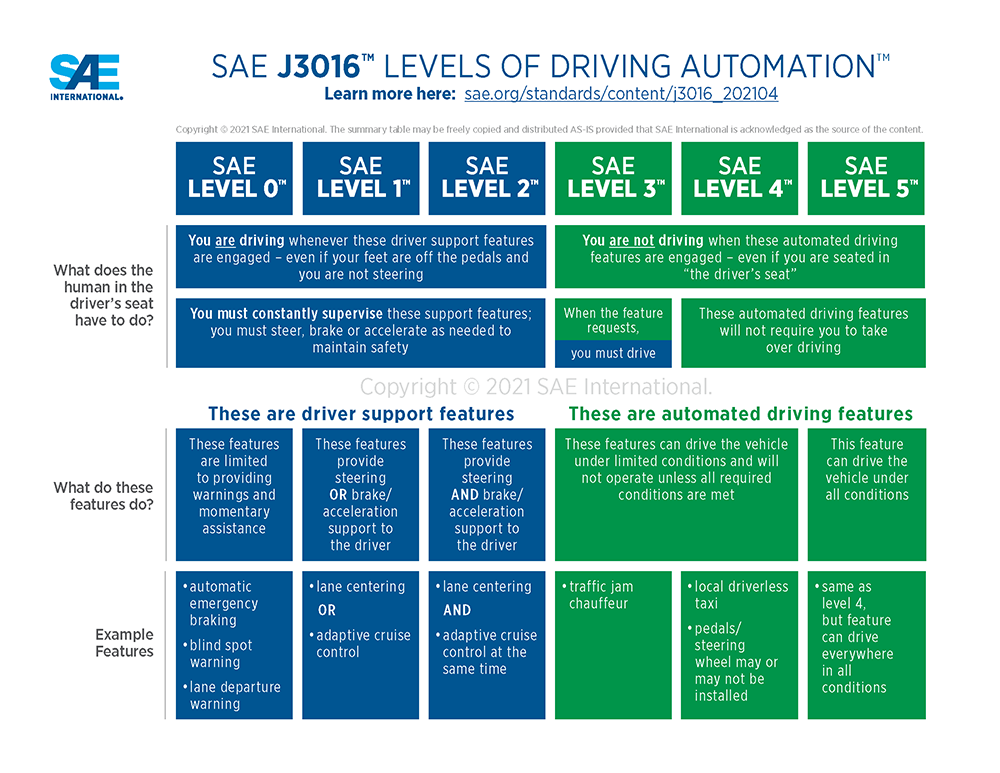
\includegraphics[width=0.9\textwidth]{images/sae-j3016-chart.png}
%   \caption{SAE J3016}
%   \label{fig:SAEJ3016}
% \end{figure}

%---------------------------------------------------------------
\subsection{Level 0 (Unified Diagnostic Services)}
%---------------------------------------------------------------

%---------------------------------------------------------------
\subsection{UDS (Unified Diagnostic Services)}
%---------------------------------------------------------------

%---------------------------------------------------------------
\subsection{UDS (Unified Diagnostic Services)}
%---------------------------------------------------------------
%---------------------------------------------------------------
\subsection{UDS (Unified Diagnostic Services)}
%---------------------------------------------------------------

%---------------------------------------------------------------
\subsection{UDS (Unified Diagnostic Services)}
%---------------------------------------------------------------

%---------------------------------------------------------------
\subsection{UDS (Unified Diagnostic Services)}
%---------------------------------------------------------------

%---------------------------------------------------------------
\section{Internal Networks}
%---------------------------------------------------------------

%---------------------------------------------------------------
\section{Controller Area Network (CAN)}
%---------------------------------------------------------------

%---------------------------------------------------------------
\subsection{J1939}
%---------------------------------------------------------------

%---------------------------------------------------------------
\subsection{OBD2}
%---------------------------------------------------------------

%---------------------------------------------------------------
\subsection{LIN (Local Interconnect Network)}
%---------------------------------------------------------------

%---------------------------------------------------------------
\subsection{UDS (Unified Diagnostic Services)}
%---------------------------------------------------------------

%---------------------------------------------------------------
\section{CAN Bus Errors}
%---------------------------------------------------------------

%---------------------------------------------------------------
\section{Data Manipulation \& Security}
%---------------------------------------------------------------

%%%%%%%%%%%%%%%%%%%%%%%%%%%%%%%%%%%%%%%%%%%%%%%%%%%%%%%%%%%%%%%%





%%%%%%%%%%%%%%%%%%%%%%%%%%%%%%%%%%%%%%%%%%%%%%%%%%%%%%%%%%%%%%%%


\chapter{III: BEATRIX (Testing System Requirements)}\addcontentsline{toc}{chapter}{III: BEATRIX}\markboth{III: BEATRIX}{III: BEATRIX}
%---------------------------------------------------------------

% The following environment can be used as a mini-introduction for a chapter. Use that any way it pleases you (or comment it out). It can contain, for instance, a summary of the chapter. Or, there can be a quotation.
\begin{chapterabstract}
	\lipsum[1]
\end{chapterabstract}

\lipsum[2][1-4]{} [1]

\lipsum[4]

%---------------------------------------------------------------
\section{Software Requirements}
%---------------------------------------------------------------

%---------------------------------------------------------------
\section{Hardware Requirements}
%---------------------------------------------------------------


%%%%%%%%%%%%%%%%%%%%%%%%%%%%%%%%%%%%%%%%%%%%%%%%%%%%%%%%%%%%%%%%





%%%%%%%%%%%%%%%%%%%%%%%%%%%%%%%%%%%%%%%%%%%%%%%%%%%%%%%%%%%%%%%%


\chapter{IV: CALEDONIA}\addcontentsline{toc}{chapter}{IV: CALEDONIA}\markboth{IV: CALEDONIA}{IV: CALEDONIA}
%---------------------------------------------------------------

% The following environment can be used as a mini-introduction for a chapter. Use that any way it pleases you (or comment it out). It can contain, for instance, a summary of the chapter. Or, there can be a quotation.
\begin{chapterabstract}
	\lipsum[1]
\end{chapterabstract}

\lipsum[2][1-4]{} [1]

\lipsum[4]

%---------------------------------------------------------------
\section{Ut enim ad minim veniam}
%---------------------------------------------------------------


%%%%%%%%%%%%%%%%%%%%%%%%%%%%%%%%%%%%%%%%%%%%%%%%%%%%%%%%%%%%%%%%





%%%%%%%%%%%%%%%%%%%%%%%%%%%%%%%%%%%%%%%%%%%%%%%%%%%%%%%%%%%%%%%%


\chapter{V: DELORES}\addcontentsline{toc}{chapter}{V: DELORES}\markboth{V: DELORES}{V: DELORES}
%---------------------------------------------------------------

% The following environment can be used as a mini-introduction for a chapter. Use that any way it pleases you (or comment it out). It can contain, for instance, a summary of the chapter. Or, there can be a quotation.
\begin{chapterabstract}
	\lipsum[1]
\end{chapterabstract}

\lipsum[2][1-4]{} [1]

\lipsum[4]

%---------------------------------------------------------------
\section{Ut enim ad minim veniam}
%---------------------------------------------------------------


%%%%%%%%%%%%%%%%%%%%%%%%%%%%%%%%%%%%%%%%%%%%%%%%%%%%%%%%%%%%%%%%





%%%%%%%%%%%%%%%%%%%%%%%%%%%%%%%%%%%%%%%%%%%%%%%%%%%%%%%%%%%%%%%%


\chapter{VI: RESULTS}\addcontentsline{toc}{chapter}{VI: RESULTS}\markboth{VI: RESULTS}{VI: RESULTS}
%---------------------------------------------------------------

% The following environment can be used as a mini-introduction for a chapter. Use that any way it pleases you (or comment it out). It can contain, for instance, a summary of the chapter. Or, there can be a quotation.
\begin{chapterabstract}
	\lipsum[1]
\end{chapterabstract}

\lipsum[2][1-4]{} [1]

\lipsum[4]

%---------------------------------------------------------------
\section{Ut enim ad minim veniam}
%---------------------------------------------------------------


%%%%%%%%%%%%%%%%%%%%%%%%%%%%%%%%%%%%%%%%%%%%%%%%%%%%%%%%%%%%%%%%










\lipsum[6-7]

\begin{figure}
\centering
%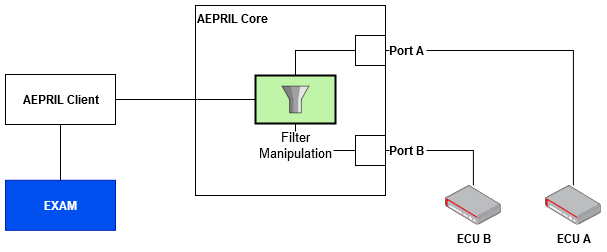
\includegraphics[scale=0.4]{pic/index}
\resizebox{\textwidth}{!}{
\begin{tikzpicture}[level/.style={sibling distance=60mm/#1}]
\node [circle,draw] (z){$n$}
  child {node [circle,draw] (a) {$\frac{n}{2}$}
    child {node [circle,draw] (b) {$\frac{n}{2^2}$}
      child {node {$\vdots$}
        child {node [circle,draw] (d) {$\frac{n}{2^k}$}}
        child {node [circle,draw] (e) {$\frac{n}{2^k}$}}
      } 
      child {node {$\vdots$}}
    }
    child {node [circle,draw] (g) {$\frac{n}{2^2}$}
      child {node {$\vdots$}}
      child {node {$\vdots$}}
    }
  }
  child {node [circle,draw] (j) {$\frac{n}{2}$}
    child {node [circle,draw] (k) {$\frac{n}{2^2}$}
      child {node {$\vdots$}}
      child {node {$\vdots$}}
    }
  child {node [circle,draw] (l) {$\frac{n}{2^2}$}
    child {node {$\vdots$}}
    child {node (c){$\vdots$}
      child {node [circle,draw] (o) {$\frac{n}{2^k}$}}
      child {node [circle,draw] (p) {$\frac{n}{2^k}$}
        child [grow=right] {node (q) {$=$} edge from parent[draw=none]
          child [grow=right] {node (q) {$O_{k = \lg n}(n)$} edge from parent[draw=none]
            child [grow=up] {node (r) {$\vdots$} edge from parent[draw=none]
              child [grow=up] {node (s) {$O_2(n)$} edge from parent[draw=none]
                child [grow=up] {node (t) {$O_1(n)$} edge from parent[draw=none]
                  child [grow=up] {node (u) {$O_0(n)$} edge from parent[draw=none]}
                }
              }
            }
            child [grow=down] {node (v) {$O(n \cdot \lg n)$}edge from parent[draw=none]}
          }
        }
      }
    }
  }
};
\path (a) -- (j) node [midway] {+};
\path (b) -- (g) node [midway] {+};
\path (k) -- (l) node [midway] {+};
\path (k) -- (g) node [midway] {+};
\path (d) -- (e) node [midway] {+};
\path (o) -- (p) node [midway] {+};
\path (o) -- (e) node (x) [midway] {$\cdots$}
  child [grow=down] {
    node (y) {$O\left(\displaystyle\sum_{i = 0}^k 2^i \cdot \frac{n}{2^i}\right)$}
    edge from parent[draw=none]
  };
\path (q) -- (r) node [midway] {+};
\path (s) -- (r) node [midway] {+};
\path (s) -- (t) node [midway] {+};
\path (s) -- (l) node [midway] {=};
\path (t) -- (u) node [midway] {+};
\path (z) -- (u) node [midway] {=};
\path (j) -- (t) node [midway] {=};
\path (y) -- (x) node [midway] {$\Downarrow$};
\path (v) -- (y)
  node (w) [midway] {$O\left(\displaystyle\sum_{i = 0}^k n\right) = O(k \cdot n)$};
\path (q) -- (v) node [midway] {=};
\path (e) -- (x) node [midway] {+};
\path (o) -- (x) node [midway] {+};
\path (y) -- (w) node [midway] {$=$};
\path (v) -- (w) node [midway] {$\Leftrightarrow$};
\path (r) -- (c) node [midway] {$\cdots$};
\end{tikzpicture}}
\caption{~Lorem ipsum dolor sit amet}\label{img:index}
\end{figure}

%---------------------------------------------------------------
\section{Ut enim ad minim veniam}
%---------------------------------------------------------------

\lipsum[2-4]

%---------------------------------------------------------------
\subsection{Ut enim ad minim veniam}
%---------------------------------------------------------------

Curabitur ligula sapien, pulvinar a vestibulum quis, facilisis vel sapien. Duis condimentum augue id magna semper rutrum. Aliquam ornare wisi eu metus. Fusce aliquam vestibulum ipsum. Vivamus ac leo pretium faucibus\ref{img:index}.

\begin{itemize}
    \item Ut enim ad minim veniam, quis nostrud
    \item Ut enim ad minim 
    \item Ut enim ad minim veniam, quis 
    \begin{itemize}
        \item Ut enim ad
        \item Ut enim ad
        \begin{itemize}
            \item Ut enim 
            \item Ut enim 
            \begin{itemize}
            \item Ut enim 
            \item Ut enim 
        \end{itemize}
        \end{itemize}
    \end{itemize}
\end{itemize}

\section{Class aptent taciti}

\lipsum[2]

\subsection{Class aptent taciti}

\lipsum[6-7]

\begin{enumerate}
    \item Ut enim ad minim veniam, quis nostrud
    \item Ut enim ad minim 
    \item Ut enim ad minim veniam, quis 
    \begin{enumerate}
        \item Ut enim ad
        \item Ut enim ad
        \begin{enumerate}
            \item Ut enim 
            \item Ut enim 
            \begin{enumerate}
            \item Ut enim 
            \item Ut enim 
        \end{enumerate}
        \end{enumerate}
    \end{enumerate}
\end{enumerate}


%---------------------------------------------------------------
\section{Ut enim ad minim veniam, quis nostrud}
%---------------------------------------------------------------

Ut enim ad minim veniam, quis nostrud exercitation ullamco laboris nisi ut aliquip ex ea commodo consequat. Nulla non arcu lacinia neque faucibus fringilla. Vestibulum erat nulla, ullamcorper nec, rutrum non, nonummy ac, erat. Aliquam erat volutpat. Proin pede metus, vulputate nec, fermentum fringilla, vehicula vitae, justo.\footnote{Ut enim ad minim veniam, quis nostrud exercitation.} Etiam dictum tincidunt diam. In laoreet, magna id viverra tincidunt, sem odio bibendum justo, vel imperdiet sapien wisi sed libero. Nulla est. Maecenas fermentum, sem in pharetra pellentesque, velit turpis volutpat ante, in pharetra metus odio a lectus. Duis aute irure dolor in reprehenderit in voluptate velit esse cillum dolore eu fugiat nulla pariatur. 

\begin{lstlisting}[caption={~Zbytečný kód},label=list:8-6,captionpos=t,float,abovecaptionskip=-\medskipamount,belowcaptionskip=\medskipamount,language=C]
    #include<stdio.h>
    #include<iostream>
    // A comment
    int main(void)
    {
        printf("Hello World\n");
        return 0;
    }
\end{lstlisting}

%%%%%%%%%%%%%%%%%%%%%%%%%%%%%%%%%
% alternative using package minted for source highlighting
% package minted requires execution with `-shell-escape'
% e.g., `xelatex -shell-escape ctufit-thesis.tex'
% \begin{listing}
% \caption{Zbytečný kód}\label{list:8-6}
% \begin{minted}{C}
%     #include<stdio.h>
%     #include<iostream>
%     // A comment
%     int main(void)
%     {
%         printf("Hello World\n");
%         return 0;
%     }
% \end{minted}
% \end{listing}
% %%%%%%%%%%%%%%%%%%%%%%%%%%%%%%%%%
Nullam feugiat, turpis at pulvinar vulputate, erat libero tristique tellus, nec bibendum odio risus sit amet ante. Aenean id metus id velit ullamcorper pulvinar. Fusce wisi. Integer lacinia. Aliquam id dolor. Pellentesque pretium lectus id turpis. Suspendisse sagittis ultrices augue. In laoreet, magna id viverra tincidunt, sem odio bibendum justo, vel imperdiet sapien wisi sed libero. Sed ac dolor sit amet purus malesuada congue. \cite{Crochemore2002}

Class aptent taciti sociosqu ad litora torquent per conubia nostra, per inceptos hymenaeos. Fusce suscipit libero eget elit. Etiam dui sem, fermentum vitae, sagittis id, malesuada in, quam. Aliquam id dolor. Curabitur bibendum justo non orci. Duis viverra diam non justo. Curabitur ligula sapien, pulvinar a vestibulum quis, facilisis vel sapien. Duis condimentum augue id magna semper rutrum. Aliquam ornare wisi eu metus. Fusce aliquam vestibulum ipsum. Vivamus ac leo pretium faucibus. \cite{Motwani2014}

%---------------------------------------------------------------
\subsection{Ut enim ad minim veniam, quis nostrud}
%---------------------------------------------------------------

Ut enim ad minim veniam, quis nostrud exercitation ullamco laboris nisi ut aliquip ex ea commodo consequat. Nulla non arcu lacinia neque faucibus fringilla. Vestibulum erat nulla, ullamcorper nec, rutrum non, nonummy ac, erat. Aliquam erat volutpat. Proin pede metus, vulputate nec, fermentum fringilla, vehicula vitae, justo. Etiam dictum tincidunt diam. In laoreet, magna id viverra tincidunt, sem odio bibendum justo. \cite{Sestakova2018} 

\begin{table}\centering
\caption[Příklad tabulky]{~Zadávání matematiky}\label{tab:matematika}
\begin{tabular}{l|l|c|c}
	Typ		& Prostředí		& \LaTeX{}ovská zkratka	& \TeX{}ovská zkratka	\tabularnewline \hline 
 	Text		& \verb|math|		& \verb|\(...\)|	& \verb|$...$|	\tabularnewline \hline
 	Displayed	& \verb|displaymath|	& \verb|\[...\]|	& \verb|$$...$$|	\tabularnewline 
\end{tabular}
\end{table}


Nulla est. Maecenas fermentum, sem in pharetra pellentesque, velit turpis volutpat ante, in pharetra metus odio a lectus. Duis aute irure dolor in reprehenderit in voluptate velit esse cillum dolore eu fugiat nulla pariatur. Nullam feugiat, turpis at pulvinar vulputate, erat libero tristique tellus, nec bibendum odio risus sit amet ante. Aenean id metus id velit ullamcorper pulvinar. 

\subsubsection{Class aptent taciti}

\begin{definition}[Optional label]
Class aptent taciti sociosqu ad litora torquent per conubia nostra, per inceptos hymenaeos. Fusce suscipit libero eget elit. Etiam dui sem, fermentum vitae, sagittis id, malesuada in, quam. Aliquam id dolor. Curabitur bibendum justo non orci.
\end{definition}

\begin{example}
Class aptent taciti sociosqu ad litora torquent per conubia nostra, per inceptos hymenaeos. Fusce suscipit libero eget elit. Etiam dui sem, fermentum vitae, sagittis id, malesuada in, quam. Aliquam id dolor. Curabitur bibendum justo non orci.
\end{example}

\begin{theorem}
Class aptent taciti sociosqu ad litora torquent per conubia nostra, per inceptos hymenaeos. Fusce suscipit libero eget elit. Etiam dui sem, fermentum vitae, sagittis id, malesuada in, quam. Aliquam id dolor. Curabitur bibendum justo non orci.
\end{theorem}

\begin{proof}
Fusce suscipit libero eget elit. Etiam dui sem, fermentum vitae, sagittis id, malesuada in, quam. Aliquam id dolor. Curabitur bibendum justo non orci.
\end{proof}

\begin{corollary}
Fusce suscipit libero eget elit. Etiam dui sem, fermentum vitae, sagittis id, malesuada in, quam. Aliquam id dolor. Curabitur bibendum justo non orci.
\end{corollary}

\begin{proposition}
Fusce suscipit libero eget elit. Etiam dui sem, fermentum vitae, sagittis id, malesuada in, quam. Aliquam id dolor. Curabitur bibendum justo non orci.
\end{proposition}

\begin{note}
Fusce suscipit libero eget elit. Etiam dui sem, fermentum vitae, sagittis id, malesuada in, quam. Aliquam id dolor. Curabitur bibendum justo non orci.
\end{note}

\begin{remark}
Fusce suscipit libero eget elit. Etiam dui sem, fermentum vitae, sagittis id, malesuada in, quam. Aliquam id dolor. Curabitur bibendum justo non orci.
\end{remark}

\begin{lemma}
Class aptent taciti sociosqu ad litora torquent per conubia nostra, per inceptos hymenaeos. Fusce suscipit libero eget elit. Etiam dui sem, fermentum vitae, sagittis id, malesuada in, quam. Aliquam id dolor. Curabitur bibendum justo non orci.
\end{lemma}

\lipsum[1-2]

\subsection{Class aptent taciti sociosqu}

\lipsum[4-5]

%---------------------------------------------------------------
\chapter{Lorem ipsum}
%---------------------------------------------------------------

\begin{chapterabstract}
	Lorem ipsum dolor sit amet, consectetuer adipiscing elit. Curabitur sagittis hendrerit ante. Class aptent taciti sociosqu ad litora torquent per conubia nostra, per inceptos hymenaeos. Cras pede libero, dapibus nec, pretium sit amet, tempor quis. Sed vel lectus. Donec odio tempus molestie, porttitor ut, iaculis quis, sem. Cras pede libero, dapibus nec, pretium sit amet, tempor quis. Sed vel lectus. 
\end{chapterabstract}

Lorem ipsum dolor sit amet, consectetuer adipiscing elit. Curabitur sagittis hendrerit ante. Class aptent taciti sociosqu ad litora torquent per conubia nostra, per inceptos hymenaeos. Cras pede libero, dapibus nec, pretium sit amet, tempor quis. Sed vel lectus. Donec odio tempus molestie, porttitor ut, iaculis quis, sem. Suspendisse sagittis ultrices augue. Donec ipsum massa, ullamcorper in, auctor et, scelerisque sed, est. In sem justo, commodo ut, suscipit at, pharetra vitae, orci. Pellentesque pretium lectus id turpis. \cite{Kopka2004}

\section{Donec odio tempus molestie}

\lipsum[2] \cite{def:1, def:2}

\subsection{Class aptent taciti}

\lipsum[2-3]

\begin{description}
\item[Kapitola 1] Lorem ipsum dolor sit amet, consectetuer adipiscing elit. Curabitur sagittis hendrerit ante. Class aptent taciti sociosqu ad litora torquent per conubia nostra, per inceptos hymenaeos. Cras pede libero, dapibus nec, pretium sit amet, tempor quis.

\item[Kapitola 2] Lorem ipsum dolor sit amet, consectetuer adipiscing elit. Curabitur sagittis hendrerit ante. Class aptent taciti sociosqu ad litora torquent per conubia nostra, per inceptos hymenaeos. Cras pede libero, dapibus nec, pretium sit amet, tempor quis.

\item[Kapitola 3] Lorem ipsum dolor sit amet, consectetuer adipiscing elit. Curabitur sagittis hendrerit ante. Class aptent taciti sociosqu ad litora torquent per conubia nostra, per inceptos hymenaeos. Cras pede libero, dapibus nec, pretium sit amet, tempor quis.

\item[Kapitola 4] Lorem ipsum dolor sit amet, consectetuer adipiscing elit. Curabitur sagittis hendrerit ante. Class aptent taciti sociosqu ad litora torquent per conubia nostra, per inceptos hymenaeos. Cras pede libero, dapibus nec, pretium sit amet, tempor quis.
\end{description}

\lipsum[2]

\section{Lorem ipsum dolor sit amet}

\lipsum[3-5]
 % include `text.tex' from `text/' subdirectory

\appendix\appendixinit % do not remove these two commands

\chapter{Nějaká příloha}


Sem přijde to, co nepatří do hlavní části.
 % include `appendix.tex' from `text/' subdirectory

\backmatter % do not remove this command

\printbibliography % print out the BibLaTeX-generated bibliography list

\chapter{Obsah přiloženého média}


	\dirtree{%
		.1 readme.txt\DTcomment{stručný popis obsahu média}.
		.1 exe\DTcomment{adresář se spustitelnou formou implementace}.
		.1 src.
		.2 impl\DTcomment{zdrojové kódy implementace}.
		.2 thesis\DTcomment{zdrojová forma práce ve formátu \LaTeX{}}.
		.1 text\DTcomment{text práce}.
		.2 thesis.pdf\DTcomment{text práce ve formátu PDF}.
	}
 % include `medium.tex' from `text/' subdirectory

\end{document}
